\documentclass[10pt,aspectratio=149]{beamer}

% All the boilerplate is in raslides.sty
% Note that this also pulls in a custom vogtwidebar.sty
\usepackage{raslides}

\author{Ji\v{r}\'i Lebl}

\institute[OSU]{%
Departemento pri Matematiko de Oklahoma {\^S}tata Universitato}

\title{BA: 3.4}

\date{}

\begin{document}

\begin{frame}
\titlepage
\end{frame}

\begin{frame}
\begin{definition}
Let $S \subset \R$, and let $f \colon S \to \R$ be a function.
Suppose for every $\epsilon > 0$ there exists a $\delta > 0$
such that whenever $x, c \in S$ and
$\abs{x-c} < \delta$, then $\abs{f(x)-f(c)} < \epsilon$.
Then we say $f$ is \emph{uniformly continuous}.
\end{definition}

\pause
Here $\delta$ does not depend on $c$, only on $\epsilon$.

\pause
\medskip

uniformly continuous \wthus continuous \quad (but not the other way round)

\pause
\medskip

\textbf{Example:}
$f \colon [0,1] \to \R$ defined by $f(x) \coloneqq x^2$ is uniformly continuous.

\pause
\medskip

Proof: Suppose $0 \leq x,c \leq 1$.  Then
$\abs{x^2-c^2}
\pause
= \abs{x+c}\abs{x-c}
\pause
\leq (\abs{x}+\abs{c}) \abs{x-c}
\pause
\leq (1+1)\abs{x-c}$.

\pause
Given $\epsilon > 0$, let $\delta \coloneqq \nicefrac{\epsilon}{2}$.

\pause
If $\abs{x-c} < \delta$, then $\abs{x^2-c^2} < \epsilon$.
\qed

\end{frame}

\begin{frame}

\textbf{Example:}
$g \colon \R \to \R$ defined by $g(x) \coloneqq x^2$ is not uniformly
continuous.

\pause
\medskip

Proof: Suppose it is.
\pause
Given $\epsilon > 0$,
$\exists$ $\delta > 0$ s.t.
if $\abs{x-c} < \delta$, then $\abs{x^2 -c^2} < \epsilon$.

\pause
For $x > 0$ let $c \coloneqq x+\nicefrac{\delta}{2}$.
\pause
Then
$\epsilon >
\abs{x^2-c^2}
\pause
= \abs{x+c}\abs{x-c}
\pause
=
(2x+\nicefrac{\delta}{2})\nicefrac{\delta}{2} 
\pause
\geq 
\delta x$.

\pause
\thus \quad $x < \nicefrac{\epsilon}{\delta}$ $\forall$ $x > 0$,
\pause
\quad
\contradiction
\qed

\pause
\medskip

\textbf{Example:}
$f \colon (0,1) \to \R$ defined by $f(x) \coloneqq \nicefrac{1}{x}$ is not
uniformly continuous.

\pause
\medskip

Proof:
For any $x,y \in (0,1)$, ~~
$\abs{\nicefrac{1}{x}-\nicefrac{1}{y}}
\pause
=
\frac{\abs{y-x}}{\abs{xy}} 
\pause
=
\frac{\abs{y-x}}{xy}$.

\pause
\medskip

Given $\epsilon > 0$,~~
$\epsilon >
\abs{\nicefrac{1}{x}-\nicefrac{1}{y}}$ ~\iffif~
$\abs{x-y} < xy \epsilon$.

\pause
Suppose $\epsilon < 1$.  Consider some $\delta > 0$.

\pause
If $x \in (0,1)$ and 
$y = x+\nicefrac{\delta}{2} \in (0,1)$,
then $\abs{x-y} = \nicefrac{\delta}{2} < \delta$.

\pause
If $\delta$ satisfies the definition, then $\nicefrac{\delta}{2} < x \bigl( x+\nicefrac{\delta}{2} \bigr) \epsilon < x$.

\pause
\medskip

$\nicefrac{\delta}{2} < x$ for all $x > 0$
\wthus
$\delta \leq 0$.
\pause
\quad
\contradiction
\qed
\end{frame}

\begin{frame}

\begin{theorem}
Let $f \colon [a,b] \to \R$ be a continuous function.  Then $f$
is uniformly continuous.
\end{theorem}

\pause
\textbf{Proof:}
Suppose $f$ is not uniformly continuous.

\pause
$\exists$ $\epsilon > 0$ and 
sequences
$\{ x_n \}_{n=1}^\infty$, $\{ y_n \}_{n=1}^\infty$ in $[a,b]$

such that
$\abs{x_n-y_n} < \nicefrac{1}{n}$ and $\abs{f(x_n)-f(y_n)} \geq
\epsilon$.

\pause
By Bolzano--Weierstrass,
$\exists$ a convergent subsequence $\{ x_{n_k} \}_{k=1}^\infty$.

\pause
Let $c \coloneqq \lim\limits_{k\to\infty} x_{n_k}$.
\pause
\quad
$a \leq c \leq b$~ as ~$a \leq x_{n_k} \leq b$ for all $k$,

\pause
\medskip

$
\abs{y_{n_k} - c}
\pause
=
\abs{y_{n_k} - x_{n_k} + x_{n_k} - c}
\pause
\leq
\abs{y_{n_k} - x_{n_k}}
+
\abs{x_{n_k}-c}
\pause
<
\nicefrac{1}{n_k} 
+
\abs{x_{n_k}-c}$.

\pause
\medskip

$\nicefrac{1}{n_k} \to 0$ and $\abs{x_{n_k}-c} \to 0$ as $k \to \infty$
\pause
\wthus $y_{n_k} \to c$ as $k \to \infty$.

\pause
\medskip

$\abs{f(x_{n_k}) - f(c)}
\pause
=
\abs{f(x_{n_k}) - f(y_{n_k}) + f(y_{n_k}) - f(c)}$

\pause
\medskip

$\qquad \geq
\abs{f(x_{n_k}) - f(y_{n_k})} - \abs{f(y_{n_k}) - f(c)}
\pause
\geq
\epsilon - \abs{f(y_{n_k})-f(c)}$

\pause
\medskip

Or \qquad
$\abs{f(x_{n_k})-f(c)} 
+
\abs{f(y_{n_k})-f(c)}
\geq
\epsilon$.

\pause
\medskip

Either $f(x_{n_k}) \not\to f(c)$ or
$f(y_{n_k}) \not\to f(c)$, otherwise the LHS would $\to 0$.

\pause
\medskip

\thus \quad $f$ is not continuous at $c$
\pause
\wthus $f$ is not continuous.
\qed

\pause
\medskip

\textbf{Remark:} See how closed and bounded is important again.

\end{frame}

\begin{frame}

\begin{definition}
A function $f \colon S \to \R$
is \emph{Lipschitz continuous}, if there exists a $K \in \R$, such that
\begin{equation*}
\abs{f(x)-f(y)} \leq K \abs{x-y} 
\qquad \text{for all } x \text{ and } y \text{ in } S.
\end{equation*}
\end{definition}

\pause
\textbf{Example:} $\sin$ and $\cos$ are Lipschitz with $K=1$ as

$\abs{\sin(x)-\sin(y)} \leq \abs{x-y} \qquad \text{and} \qquad
\abs{\cos(x)-\cos(y)} \leq \abs{x-y}$.


\pause
\begin{proposition}
A Lipschitz continuous function is uniformly continuous.
\end{proposition}

\pause
\textbf{Proof:}
Suppose $f \colon S \to \R$ and $K$ are such that

$\abs{f(x)-f(y)} \leq K \abs{x-y}$ for all $x, y$ in $S$.

\pause
\medskip

Let $\epsilon > 0$ be given.
\pause
\quad
Take $\delta \coloneqq \nicefrac{\epsilon}{K}$.

\pause
\medskip

For all $x,y \in S$ such that
$\abs{x-y} < \delta$,
\pause
\quad
$\abs{f(x)-f(y)}
\pause
\leq K \abs{x-y}
\pause
< K \delta
\pause
= K \frac{\epsilon}{K}
\pause
=
\epsilon$.

\pause
\medskip

\thus \quad $f$ is uniformly continuous.
\qed

\end{frame}

\begin{frame}
Geometric interpretation of Lipschitz:

\pause
\medskip

Suppose $f$ is Lipschitz with constant $K$.

\pause
\medskip

If $x \not= y$, then
\quad
$\displaystyle
\abs{\frac{f(x)-f(y)}{x-y}} \leq K$.

\pause
\vspace*{-0.3in}
\hspace*{2.5in}
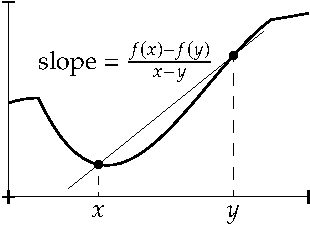
\includegraphics{../figures/lipschitzfig}

\vspace*{-1.0in}

$\frac{f(x)-f(y)}{x-y}$ is the slope of the line
between

$\bigl(x,f(x)\bigr)$ and $\bigl(y,f(y)\bigr)$,
~
the \emph{secant line}.

\pause
\medskip

$f$ is Lipschitz

\wiffif

every secant line has $\abs{\text{slope}} \leq K$.

\end{frame}

\begin{frame}
\textbf{Example:}
$f \colon [1,\infty) \to \R$ given by $f(x) \coloneqq \sqrt{x}$
is Lipschitz continuous.

\pause
\medskip

Proof:
$
\abs{\sqrt{x}-\sqrt{y}}
\pause
= 
\abs{\frac{x-y}{\sqrt{x}+\sqrt{y}}}
\pause
=
\frac{\abs{x-y}}{\sqrt{x}+\sqrt{y}}$.

\pause
\medskip

As $x \geq 1$ and $y \geq 1$, we see that $\frac{1}{\sqrt{x}+\sqrt{y}}
\leq \frac{1}{2}$.

\pause
Therefore, \quad
$\abs{\sqrt{x}-\sqrt{y}}
\pause
= 
\abs{\frac{x-y}{\sqrt{x}+\sqrt{y}}}
\pause
\leq
\frac{1}{2}
\abs{x-y}$.
\qed

\pause
\medskip

\textbf{Example:}
$g \colon [0,\infty) \to \R$ given by
$g(x) \coloneqq \sqrt{x}$ is not Lipschitz continuous.

\pause
\medskip

Proof:  Suppose $K$ exists (assume $K>0$), s.t. 
$\abs{\sqrt{x}-\sqrt{y}} 
\leq
K \abs{x-y}$ $\forall$ $x,y \geq 0$.

\pause
\medskip

Set $y=0$ \wthus $\sqrt{x} \leq K x$.

\pause
For $x > 0$, ~$\nicefrac{1}{K} \leq \sqrt{x}$ ~~ or ~~ $\nicefrac{1}{K^2} \leq x$.

\pause
This can't be true for all $x > 0$ \wthus no $K$ exists
\pause
\wthus
$g$ not Lipschitz.
\qed

\pause
\medskip

\textbf{Remark:} $g$ is uniformly continuous (exercise), but not Lipschitz.

\end{frame}

\end{document}
